\section{Auswertung}
Um die Funktionsweise des Germanium-Detektors zu untersuchen, werden nun im Folgenden die aufgenommenen Spektren ausgewertet.

\subsection{Kalibrierung und Effizienzbestimmung des Germanium-Detektors}

Zur Kalibrierung des Germanium-Detektors wird das Spektrum eines $^{152}$Eu-Strahlers untersucht. Hierbei
werden im aufgenommenen Spektrum die Peaks detektiert und dann den im Energiespektrum von $^{152}$Eu, die der
Versuchsanleitung \cite{Q1} entnommen wurden, hervorstechenden Energiewerten zugeordnet. Das
$^{152}$Eu-Spektrum mit den detektierten Peaks ist in
Abbildung \ref{abb:Europiumspektrum} zu sehen. Die abbildung des Energiespektrums wurde, wie alle folgenden Plots in der Form bearbeitet, als
dass sie jeweils nur die für die Auswertung relevanten Ausschnitte aus dem Spektrum darstellen.
Die fertige Zuordnung von Binwerten zu den Energien ist in Tabelle \ref{tab:Kali} zu sehen.
\FloatBarrier
\begin{figure}
    \centering
    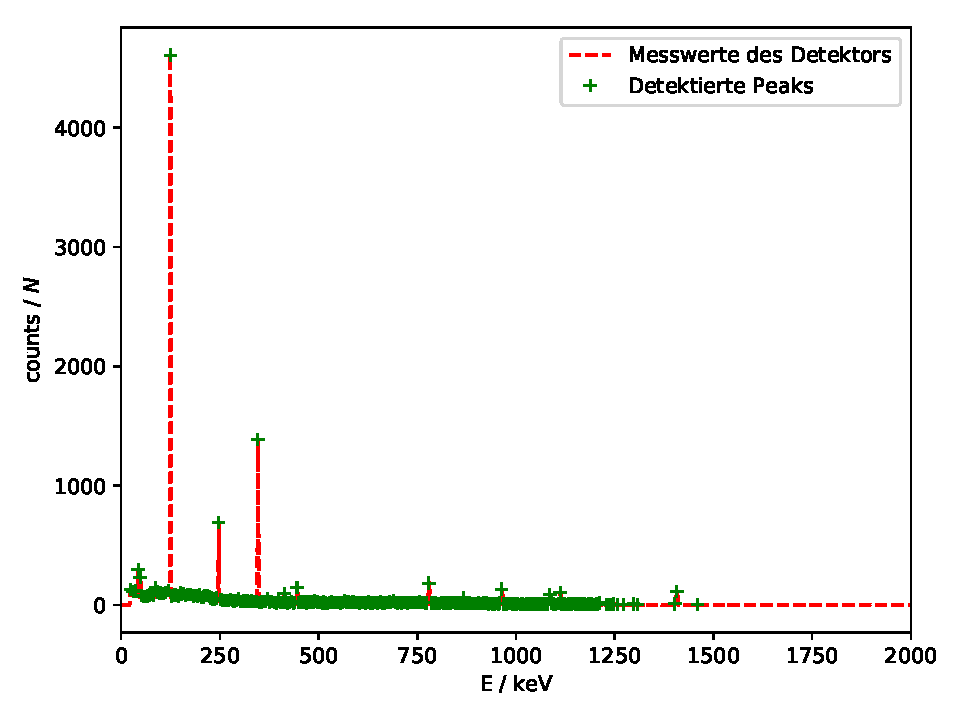
\includegraphics[scale=0.7]{Detektormesswerte.pdf}
    \caption{$^{152}$Eu-Spektrum mit detektierten Peaks.}
    \label{abb:Europiumspektrum}
\end{figure}
\FloatBarrier

\begin{table}
    \centering
    \caption{Werte zur Kalibrierung des Germanium-Detektors.}
    \label{tab:Kali}
    \begin{tabular}{ c c c c }
        \toprule
        {$\text{E}_{\gamma}$ / $\si{\kilo \electronvolt}$} & { Wahrscheinlichkeit W} & {zugeordneter Bin-Index} & {Peakhöhe}     \\
        \midrule
        121,78 &    28,6 &  309  & 4608 \\
        244,70 &     7,6 &   614  & 692 \\
        295,94 &    0,4 &   741  & 35 \\
        344,30 &     26,5 &  861  & 1388 \\
        411,12 &    2,2 &   1027 & 94 \\
        443,96 &    3,1 &   1108 & 149 \\
        678,00 &     2,0 &   1689 & 29 \\
        688,67 &    0,9 &   1715 & 35 \\
        778,90 &     12,9 &  1939 & 184 \\
        867,37 &    4,2 &   2159 & 62 \\
        964,08 &    14,6 &  2398 & 134 \\
        1005,30 &    0.6 &   2500 & 15 \\
        1085,90 &    10,2 &  2702 & 85 \\
        1112,10 &    13,6 &  2766 & 106 \\
        1299,10 &    1,6 &   3229 & 10 \\
        1408,00 &    21,0 &  3502 & 116 \\
        1457,60 &    0,5 &   3633 &   6 \\
        \bottomrule
    \end{tabular}
\end{table}
\FloatBarrier

\noindent Mittels der Zuordnung der Bin-Indizes zu den Energien kann nun eine lineare Ausgleichsrechunung der Form
\begin{align*}
    E(K) = m \cdot K + n
\end{align*}
durchgeführt werden. Hierbei beschreibt K die Kanalnummer.
Für die Werte des linearen Fits ergibt sich dann:

\begin{align*}
    m &= \SI{0,4018 \pm 0,0007}{\kilo \electronvolt} \\
    n &= \SI{0,2(16)}{\kilo \electronvolt}
\end{align*}

\noindent Die Wertepaare aus bestehend aus dem Bin-Index und der zugeordneten Energie aus den Literaturwerten sind gemeinsam mit dem linearen Fit in Abbildung \ref{abb:linfit} zu sehen.

\FloatBarrier
\begin{figure}
    \centering
    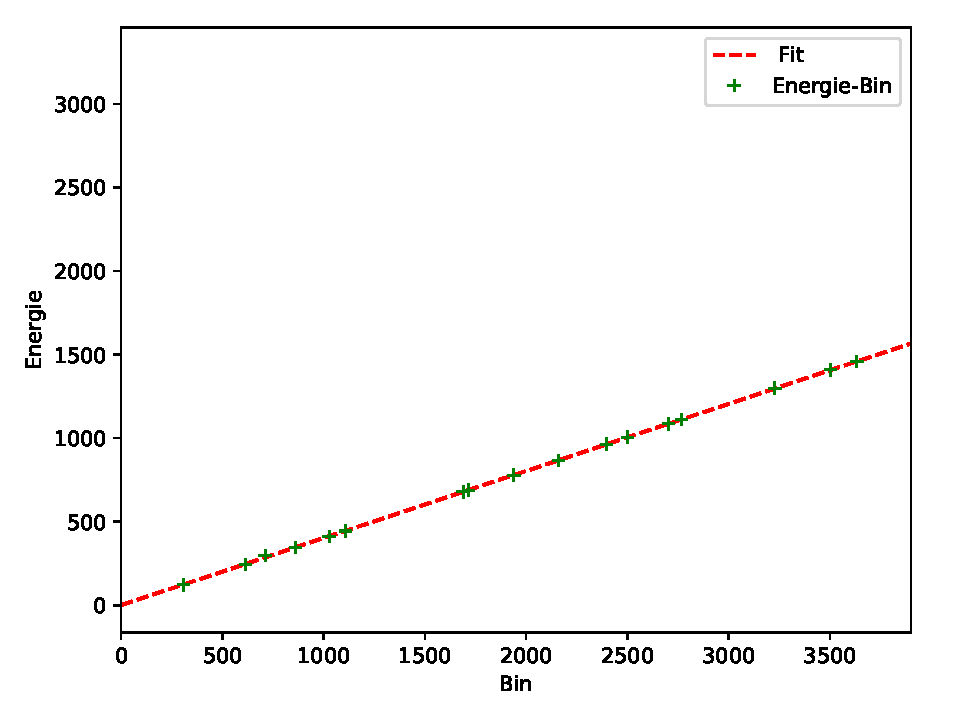
\includegraphics[scale=0.7]{Kalibrierung.pdf}
    \caption{Energiekalibrierung des Germanium-Detektors.}
    \label{abb:linfit}
\end{figure}
\FloatBarrier

\noindent Um die Effizienz des Germanium-Detektors gemäß Formel \ref{eq:effizienz} zu bestimmen, müssen zunächst die Parameter A, Z, W und $\Omega$ ermittelt werden.
Die Aktivität A der Probe am Versuchstag, dem 07.11.2018, lässt sich mit den Angaben zur Halbwertszeit von $^{152}$Eu ($t_{1/2}=\SI{4943(5)}{\days}$) und der Aktivität am 01.10.2000: $\text{A}_0= \SI{4130(60)}{\becquerel}$ aus der Versuchsanleitung \cite{Q1} einfach berechnen:
\begin{align*}
    \text{A} &= \text{A}_0 \exp \left(-\frac{\ln(2) \Delta t}{t_{1/2}}\right)
    &= \SI{1634(24)}{\becquerel}
\end{align*}
Das Raumwinkelelement $\frac{\Omega}{4 \pi}$ berechnet sich nach Gleichung \ref{eq:Omega} mit dem Parameter $a$ für den Abstand zwischen Quelle und Absorptionspunkt ($a=\SI{8,81}{\centi\meter}$) und $r$ für die halbe Breite des Germanium-Detektors ($r= \SI{2,25}{\centi \meter}$). Die Wahl für $a$ ergibt sich aus der Angabe aus der Anleitung zum Versuch \cite{Q1}, dass der wahrscheinlichste Absorptionspunkt im Germanium $\SI{1,5}{\centi \meter}$ unter der Aluminiumhaube liegt und der Höhe des Abstandshalters zwischen Probe und Detektor ($\SI{7,31}{\centi \meter}$).
Mit Hilfe dieser Parameter berechnet sich das Raumwinkelelement zu:
\begin{align*}
    \frac{\Omega}{4 \pi} = 0,016 \; .
\end{align*}

\noindent Die Peakinhalte zu den angegebenen Energien werden bestimmt, indem Gaußfits über jeden Peak gelegt werden. Die Gaußfits besitzen folgende Form:
\begin{equation*}
    f(K) = h \cdot \exp\left(\frac{-(K-\mu)^2}{2\sigma^2}\right) +a \;
\end{equation*}
Hierbei beschreibt $h$ die Höhe des Peaks, $\mu$ den Mittelwert, mit dem der zuvor zugeordnete Bin-Index korrigiert wird, $\sigma$ die Standardabweichung, $K$ die Kananummer und $a$ die Untergrundstrahlung.
Die Peakinhalte $Z_i$ werden dann über Integration über die Gaußkurven berechnet:
\begin{equation*}
    Z_i = \sqrt{2\pi} \cdot h_i \cdot \sigma_i
\end{equation*}
\FloatBarrier
Die sich ergebenden Parameter und Ergebnisse für die Peakinhalte $Z_i$, sowie die berechneten Effizienzen ($Q(E_i)$) sind in den Tabellen \ref{tab:effizienz1} und \ref{tab:effizienz2} zu sehen.
Anschließend wird ein nicht linearer Fit der Werte für $E_i$ und $Q(E_i)$ vorgenommen, der folgende Form besitzt:
\begin{equation*}
    Q(E) = a \cdot \left( \frac{E}{\si{1}{\kilo \electronvolt}}\right)^{b}
\end{equation*}
Hierbei ist zu beachten, dass lediglich Energien berücksichtigt werden, die größer als $\SI{150}{\kilo \electronvolt}$ sind.
Für die Fitparameter ergeben sich folgende Werte:
\begin{align*}
 a &= \SI{1.21(49}{}
 b &= \SI{-1.10(6)}{}
\end{align*}

Die Wertepaare, als auch die gefittete Potenzfunktion, sind in Abbildung \ref{abb:effizienz} zu sehen.
\FloatBarrier
\begin{table}
    \centering
    \caption{Werte zur Effizienbestimmung aus den Gaußfits}
    \label{tab:effizienz1}
    \begin{tabular}{ c c c c }
        \toprule
        {$\sigma_i$}            & {$\mu_i$}             & {$h_i$}           & {$a_{i}$}         \\
        \midrule

        1.130 \pm  0.005        & 308.800 \pm  0.005    & 4579 \pm  18      & 90 \pm  4         \\
        1.293 \pm  0.014        & 613.806 \pm  0.013    & 652 \pm  6        & 38.5 \pm  1.3     \\
        1.40 \pm  0.28          & 741.45 \pm  0.27      & 28 \pm  5         & 26.2 \pm  1.1     \\
        1.547 \pm  0.014        & 860.911 \pm  0.013    & 1349 \pm  10      & 20.1 \pm  2.6     \\
        1.80 \pm  0.08          & 1026.69 \pm  0.07     & 80.6 \pm  2.9     & 17.5 \pm  0.8     \\
        1.58 \pm  0.06          & 1108.16 \pm  0.06     & 125 \pm  4        & 15.8 \pm  1.0     \\
        1.3 \pm  0.4            & 1689.2 \pm  0.4       & 12.0 \pm  3.5     & 14.5 \pm  0.8     \\
        1.01 \pm  0.27          & 1715.07 \pm  0.26     & 19 \pm  4         & 14.6 \pm  0.9     \\
        2.58 \pm  0.06          & 1939.19 \pm  0.05     & 166.9 \pm  3.1    & 12.0 \pm  1.1     \\
        2.44 \pm  0.17          & 2158.90 \pm  0.16     & 47.7 \pm  2.7     & 13.0 \pm  1.0     \\
        3.24 \pm  0.13          & 2398.51 \pm  0.11     & 123 \pm  4        & 6.5 \pm  1.7      \\
        1.01 \pm  0.34          & 2500.23 \pm  0.33     & 9.1 \pm  2.6      & 6.1 \pm  0.5      \\
        3.18 \pm  0.14          & 2700.87 \pm  0.12     & 75.9 \pm  2.6     & 9.8 \pm  1.1      \\
        3.35 \pm  0.13          & 2766.14 \pm  0.11     & 98.5 \pm  3.0     & 5.7 \pm  1.4      \\
        0.84 \pm  0.22          & 3228.31 \pm  0.21     & 9.1 \pm  2.0      & 2.37 \pm  0.35    \\
        3.63 \pm  0.15          & 3501.10 \pm  0.12     & 103.2 \pm  3.2    & 2.4 \pm  1.6      \\
        6.2 \pm  1.6            & 3630.4 \pm  1.0       & 3.4 \pm  0.6      & 0.0 \pm  0.6      \\

        \bottomrule
    \end{tabular}
\end{table}

\FloatBarrier
\begin{table}
    \centering
    \caption{Werte zur Effizienzbestimmung aus den Gaußfits}
    \label{tab:effizienz2}
    \begin{tabular}{ c c c }
        \toprule
        {$Z_i$}             & {$E_i$ / $\si{\kilo\electronvolt}$} & {$Q(E_i)$ }               \\
        \midrule
        12970 \pm  80       & 122.1847 \pm  0.0021                & -                         \\
         2113 \pm  29       & 244.989 \pm  0.005                  & 0.284 \pm  0.006          \\
           97 \pm  25       & 296.38 \pm  0.11                    & 0.25 \pm  0.07            \\
         5230 \pm  60       & 344.481 \pm  0.005                  & 0.202 \pm  0.004          \\
          364 \pm  21       & 411.230 \pm  0.030                  & 0.169 \pm  0.010          \\
          496 \pm  24       & 444.032 \pm  0.022                  & 0.164 \pm  0.008          \\
           39 \pm  17       & 677.97 \pm  0.17                    & 0.020 \pm  0.009          \\
           49 \pm  17       & 688.39 \pm  0.11                    & 0.055 \pm  0.019          \\
         1080 \pm  32       & 778.630 \pm  0.022                  & 0.0856 \pm  0.0028        \\
          292 \pm  26       & 867.09 \pm  0.06                    & 0.071 \pm  0.007          \\
         1000 \pm  50       & 963.57 \pm  0.05                    & 0.070 \pm  0.004          \\
           23 \pm  10       & 1004.52 \pm  0.13                   & 0.039 \pm  0.017          \\
          604 \pm  34       & 1085.31 \pm  0.05                   & 0.0606 \pm  0.0035        \\
          830 \pm  40       & 1111.58 \pm  0.05                   & 0.0621 \pm  0.0032        \\
           19 \pm  6        & 1297.67 \pm  0.08                   & 0.012 \pm  0.004          \\
          940 \pm  50       & 1407.50 \pm  0.05                   & 0.0458 \pm  0.0024        \\
           53 \pm  17       & 1459.6 \pm  0.4                     & 0.108 \pm  0.035          \\
        \bottomrule
    \end{tabular}
\end{table}
\FloatBarrier
\begin{figure}
    \centering
    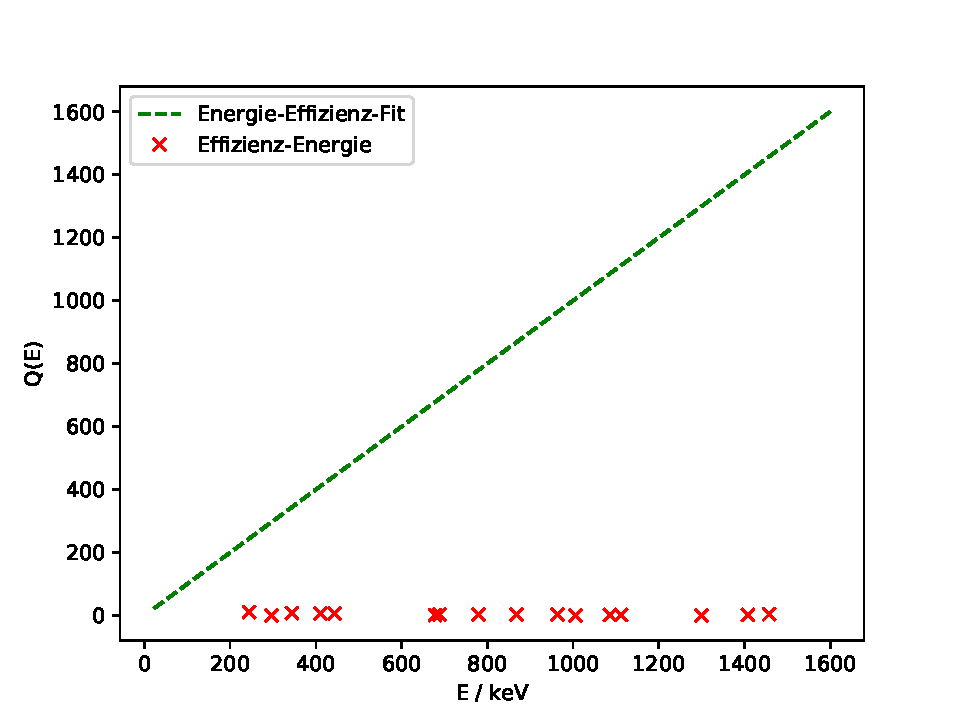
\includegraphics[scale=0.7]{effizienz.pdf}
    \caption{Effizienz des Germanium-Detektors gegen die Energie aufgetragen.}
    \label{abb:effizienz}
\end{figure}
\FloatBarrier
\subsection{Untersuchung der Halbwertsbreite des Photopeaks eines $^{137}$Cs-Strahlers}

Um die Halbwertsbreite des Photopeaks eines $^{137}$Cs-Strahlers zu untersuchen,
wird das Spektrum eines monochromatischen Gammastrahlers, das von $^{137}$Cs,
aufgenommen. Das erhaltene Spektrum ist zusammen mit den detektierten Peaks in
Abbildung \ref{abb:Cs_peaks} zu sehen. Die für die Auswertung wichtigen Peaks sind der
Photopeak, der Rückstreupeak sowie die Compton-Kante. Die erhaltenen Werte für die
Bin-Indizes sowie die zugehörigen Energiewerte sind in Tabelle \ref{tab:Cs_peaks}
dargestellt.
\FloatBarrier
\begin{table}
    \centering
    \caption{Lage und Energie der charakteristischen Peaks des $^{137}$Cs-Strahlers}
    \label{tab:Cs_peaks}
    \begin{tabular}{ c c c }
        \toprule
        & {Bin-Index} & {Energie $E_i$}      \\
        \midrule
        {Rückstreupeak} & 486  & 195,44      \\
        {Compton-Kante} & 1164 & 467,87      \\
        {Photopeak}     & 1648 & 662,35      \\
        \bottomrule
    \end{tabular}
\end{table}
\FloatBarrier
Bei der Analyse der Lage der Peaks ist zu erkennen, dass die Energie des Photopeaks mit $\SI{662,35}{\kilo \electronvolt}$ sehr nah am Theoriewert ($\SI{661,59}{\kilo \electronvolt}$) liegt \ref{Q3}.
Der Theoriewert für Rückstreupeak und Compton-Kante kann wie folgt aus der Energie des Photopeaks berechnet werden:
\begin{align*}
    E_{\text{comp,theo}} &= E_\text{photo} \frac{2\epsilon}{1+2\epsilon} = \SI{477,98}{\kilo\electronvolt} \\ \Delta E_\text{comp} &= \SI{2,11}{\percent} \\
    E_{\text{rück,theo}} &= E_\text{photo} \frac{1}{1+2\epsilon} = \SI{184,38}{\kilo\electronvolt} \\
    \Delta E_\text{rück} &= \SI{6,00}{\percent}
\end{align*}
In dieser Berechnung beschreibt $\epsilon$ das Verhältnis zwischen der Energie des Photopeaks $E_\text{photo}$ zur Ruheenergie eines Elektrons: $\epsilon = \frac{E_\text{photo}}{m_e c^2}$.

\noindent Im Anschluss daran wird überprüft, ob der Photopeak Gauß-förmig ist.
Dies geschieht, indem die Flanken des Peaks mittels linearer Ausgleichsrechnung approximiert werden. Somit kann leicht die Halberts- und Zehntelwertsbreite ermittelt werden. Stehen die beiden Breiten in einem bestimmten Verhältnis zueinander, so kann davon ausgegangen werden, dass der Peak Gauß-förmig ist.
Die lineare Ausgleichsrechung hat die Form $F(K) = m \cdot K + n$. Hierbei beschreibt $K$ die Kanalnummer.
Für die Parameter links (l) und rechts (r) am Peak ergeben sich folgende Werte:
\begin{align*}
    m_l &= 0,0028 \pm 0,0003 & m_r &= -0,00213 \pm 0,00018 \\
    n_l &= 1641,9 \pm 0,4    & n_r &=  1652,94 \pm 0,25
\end{align*}
Die Berechnung der Halbwerts- und Zehntelwertsbreite erfolgt mittels folgender Rechnung:
\begin{align*}
    \Delta_{h} = m_r E h + n_r - (m_l E h + n_l) \; \text{mit} \; h \in \{0,1 \; , \; 0,5\} \;
\end{align*}
und ergibt folgende Werte:
\begin{align*}
    \Delta_{0,5} &= \SI{2,45(23)}{\kilo \electronvolt}\\    %An Kommata denken.
    \Delta_{0,1} &= \SI{4,16(18)}{\kilo \electronvolt} \; . %An Kommata denken.
\end{align*}
Für eine Gaußverteilung gilt:
\begin{align*}
    \Delta_{0,1} &= 1,823 \cdot \Delta_{0,5} \\
                 &= \SI{4,3(4)}{\kilo \electronvolt} \; .
\end{align*}
Der mit Hilfe der Halbwertsbreite berechnete Wert für die Zehntelwertsbreite weicht
dabei lediglich um $\SI{4}{\percent}$ von dem experimentell ermittelten ab, weshalb
davon auszugehen ist, dass eine Gaußverteilung vorliegt.
\FloatBarrier
\begin{figure}
    \centering
    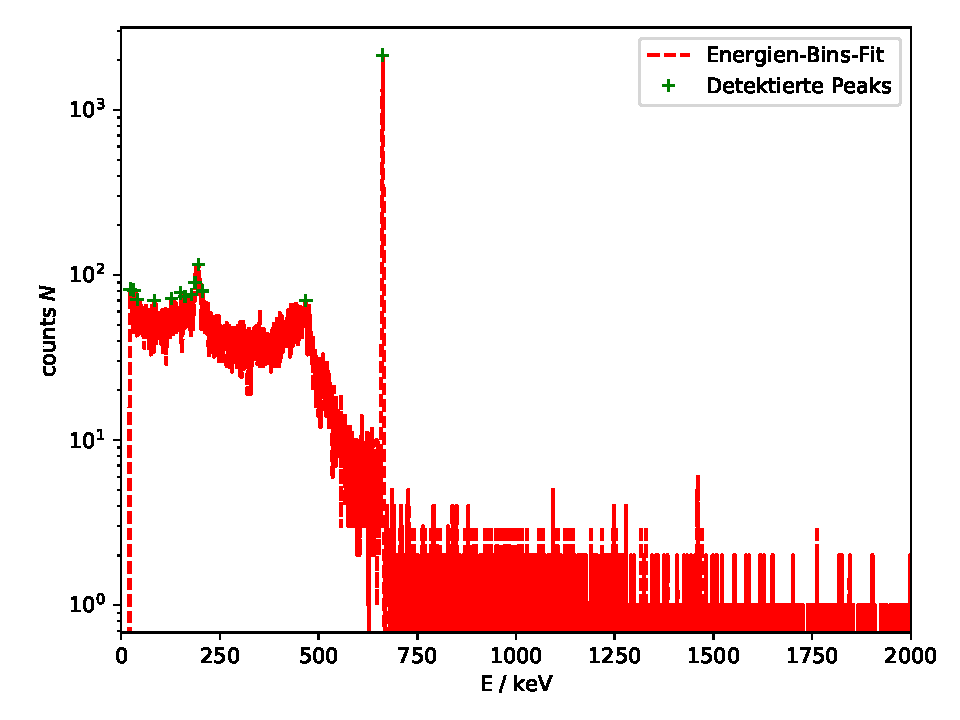
\includegraphics[scale=0.7]{Cs_fit.pdf}
    \caption{Comptonkontinuum und Photopeak des $^{137}$Cs-Strahlers.}
    \label{abb:Cs_peaks}
\end{figure}
\FloatBarrier

\noindent Im letzten Teil wird der Inhalt des Photopeaks und des Comptonkontinuums mit der Absorptionswahrscheinlichkeit für Photo- und Comptoneffekt verglichen.
Die Extinktionskoeffizienten $\mu$ ergeben sich aus der Versuchsanleitung \cite{Q1}, woraus anschließend die Absorptionswahrscheinlichkeiten berechnet werden können ($p = 1-\exp(-\mu l)$). Hierbei beschreibt $l= \SI{3,9}{\centi \meter}$ die Länge des Detektors.
\begin{align*}
    \mu_{\text{comp}} &= \SI{0,38}{\centi \meter} \\
    p_{\text{comp}} &= \SI{77,28}{\percent}\\
    \mu_{\text{photo}} &= \SI{0,002}{\centi \meter} \\
    p_{\text{photo}} &= \SI{0,78}{\percent}
\end{align*}
Der Inhalt des Photopeaks wird auch in diesem Teil des Versuchs ermittelt, indem er mit einem Gaußfit gefittet wird. Das Comptonkontinuum hingegen wird mit einer Funktion gefittet, die proportional zum zugehörigen Wirkungsquerschnitt \ref{eq:WQ} ist. Die Proportionalitätskonstante wird durch das Verhältnis von der Zählrate an der Compton-Kante zum Wert der Funktion definiert.
Die Funktion, mit der das Comptonkontinuum gefittet wurde, wird anschließend mittels der Funktion "quad" aus scipy.integrate integriert, sodass sich für den Inhalt des Comptonkontinuums und des Photopeaks folgende Werte ergeben:
\begin{align*}
    Z_{\text{comp}}  &= 21150,22 \\
    Z_{\text{photo}} &= \SI{12010(100)}{}
\end{align*}
Es ist zu sehen, dass der Inhalt des Photopeaks zwar kleiner als der des  Comptonkontinuums ist, jedoch nicht derart kleiner, wie es die deutlich unterschiedlich großen Absorptionswahrscheinlichkeiten hätten erwarten lassen.
Somit kann davon ausgegangen werden, dass die Elektronen nicht nur einmalig Energie beim Comptoneffekt abgeben, sondern mehrfach, bevor sie dann ihre komplette Energie im durch den Photoeffekt verlieren.
Der Extinktionskoeffizient \ref{abb:1} ist höher für den Photoeffekt, was diesen wahrscheinlicher macht.

\subsection{Aktivität einer $^{133}$Ba-Quelle}

\noindent In diesem Teil des Versuchs wird das Spektrum einer $^{133}$Ba-Strahlers untersucht. Dafür werden die Peaks zunächst analog zum ersten Teil des Versuchs detektiert, anschließend Gauß-gefittet, die Peakinhalte ermittelt, indem über die Gaußfits integriert wird. Die zugeordneten Bin-indizes, sowie gefitteten Energien sind in Tabelle \ref{tab:BaTab} dargestellt.
\FloatBarrier
\begin{table}
    \centering
    \caption{Zugeordnete Peaks und Bins einer $^{133}$Ba-Quelle. }
    \label{tab:BaTab}
    \begin{tabular}{cccc}
        \toprule
        {E / keV} & { W } & zugeordneter Bin-Index & gefittete Energie \\
        \midrule
        53.16   &   2.2   &   139.0  &    55.86\pm0.07 \\
        79.62   &   2.6   &   192.0  &    71.3\pm2.4 \\
        81.0    &   34.1  &   208.0  &    83.575\pm0.008 \\
        160.61  &   0.6   &   405.0  &    163.00\pm0.09 \\
        302.85  &   18.3  &   758.0  &    304.7824\pm0.0026 \\
        356.02  &   62.1  &   890.0  &    357.8077\pm0.0030 \\
        383.85  &   8.9   &   960.0  &    385.616\pm0.010 \\
        \bottomrule
    \end{tabular}
\end{table}
\FloatBarrier

\noindent Mit Hilfe der Formel für die Ermittlung der Effizienz \ref{eq:effizienz}, kann so ein Wert für die Aktivität der Bariumquelle ermittelt werden. Hierbei ist darauf zu achten, da nur Werte mit einer Energie $E_i$ größer als $\SI{150}{\kilo \electronvolt}$, da nur für diese Werte die Effizienz bestimmt werden kann.
Die Werte, die sich für die Bin-Indizes, die Standardabweichung, die Höhe der Peaks, die Peakinhalte, die Energie, sowie die Aktivität der Quelle ergeben, sind in den Tabellen \ref{tab:BaAkt} \ref{tab:BaAkt2} dargestellt.
Die Detektormesswerte, sowie die ermittelten Peaks der Bariumquelle sind in Abbildung \ref{abb:BaPlot} dargestellt.
\FloatBarrier
\begin{table}
    \centering
    \caption{Ergebnisse zur bestimmung der Aktivität der $^{133}$Ba-Quelle aus den Gaußfits der Peaks.}
    \label{tab_BaAkt}
    \begin{tabular}{ c c c }
        \toprule
        {$\sigma_{\text{ba}}$} & {$h_i$} &  {$a_i$}                     \\
        \midrule
        0.85 \pm 0.19     & 64 \pm 12              &     71.6 \pm 1.5   \\
        -13 \pm 9         & -470 \pm 210           &     470 \pm 170    \\
        1.081 \pm 0.020   & 3490\pm 50             &     84 \pm 8       \\
        0.79 \pm 0.23     & 84 \pm 21              &     89.3 \pm 2.6   \\
        1.384 \pm 0.007   & 930 \pm 4              &     12.9 \pm 0.7   \\
        1.513 \pm 0.008   & 2403 \pm 10            &     8.0 \pm 1.9    \\
        1.657 \pm 0.027   & 286 \pm 4              &     2.9 \pm 0.8    \\
        \bottomrule
    \end{tabular}
\end{table}
\FloatBarrier
\begin{table}
    \centering
    \caption{Ergebnisse zur bestimmung der Aktivität der $^{133}$Ba-Quelle aus den Gaußfits der Peaks.}
    \label{tab:BaAkt2}
    \begin{tabular}{ c c c }
        \toprule
        {Bin-Index} & {Peakinhalt $Z_i$} & {Aktivität $A_i$} \\
        \midrule
        138.62 \pm 0.17   & 130 \pm 40       & - \\
        170 \pm 8         & 11000 \pm 1000   & - \\
        207.604 \pm 0.017 & 9480 \pm 200     & - \\
        405.26 \pm 0.23   & 190 \pm 70       & - \\
        758.119 \pm 0.006 & 3227 \pm 18         & 1858\pm11 \\
        890.082 \pm 0.007 & 9120 \pm 50         & 1633\pm10 \\
        959.288 \pm 0.023 & 1187 \pm 22         & 1525\pm28 \\
        \bottomrule
    \end{tabular}
\end{table}
\FloatBarrier
Die erhaltenen Werte für die Aktivität werden anschließend gemittelt, wodurch sich folgender Wert für die Aktivität der $^{133}$Ba-Quelle ergibt:
\begin{align*}
    A_\text{Ba} = \SI{1672\pm18}{\becquerel}
\end{align*}
\FloatBarrier
\begin{figure}
    \centering
    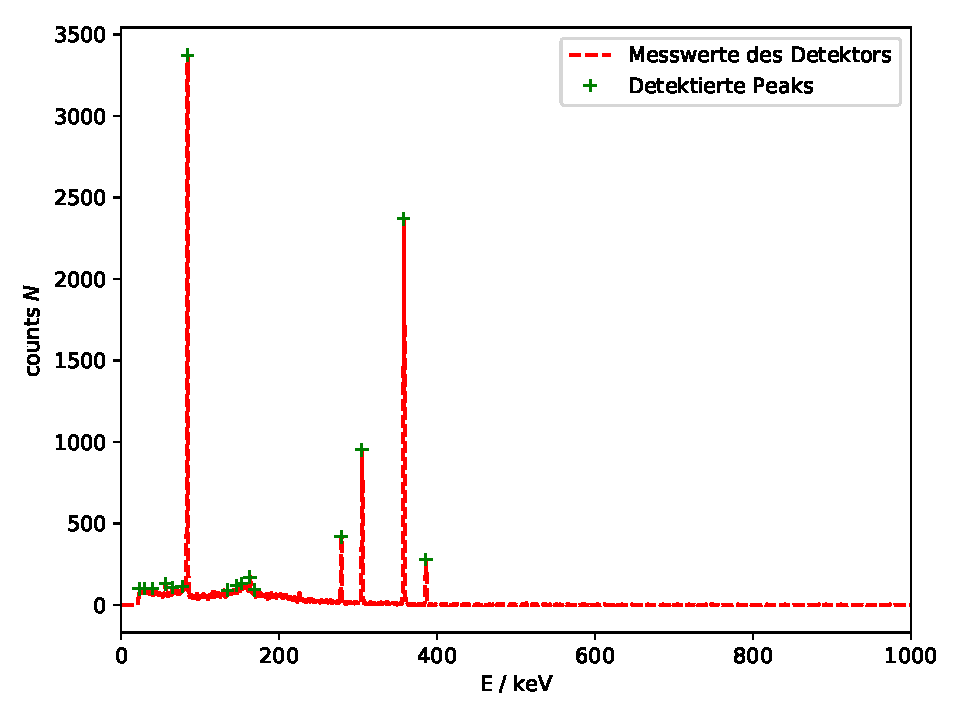
\includegraphics[scale=0.7]{Ba_plot_peaks.pdf}
    \caption{Spektrum mit detektierten Peaks einer $^{133}$Ba-Quelle.}
    \label{abb:BaPlot}
\end{figure}
\FloatBarrier
\subsection{Aktive Nuklide eines unbekannten Strahlers}
Im finalen Teil des Versuchs wird eine unbekannte Substanz im Germanium-Detektor analysiert. Das Spektrum, sowie die detektierten Peaks sind in Abbildung \ref{abb:unbekannt} zu sehen. Die Position, sowie die Höhe und zugehörige Energie sind in Tabelle \ref{tab:unbekannt} zu sehen.
\FloatBarrier
\begin{figure}
    \centering
    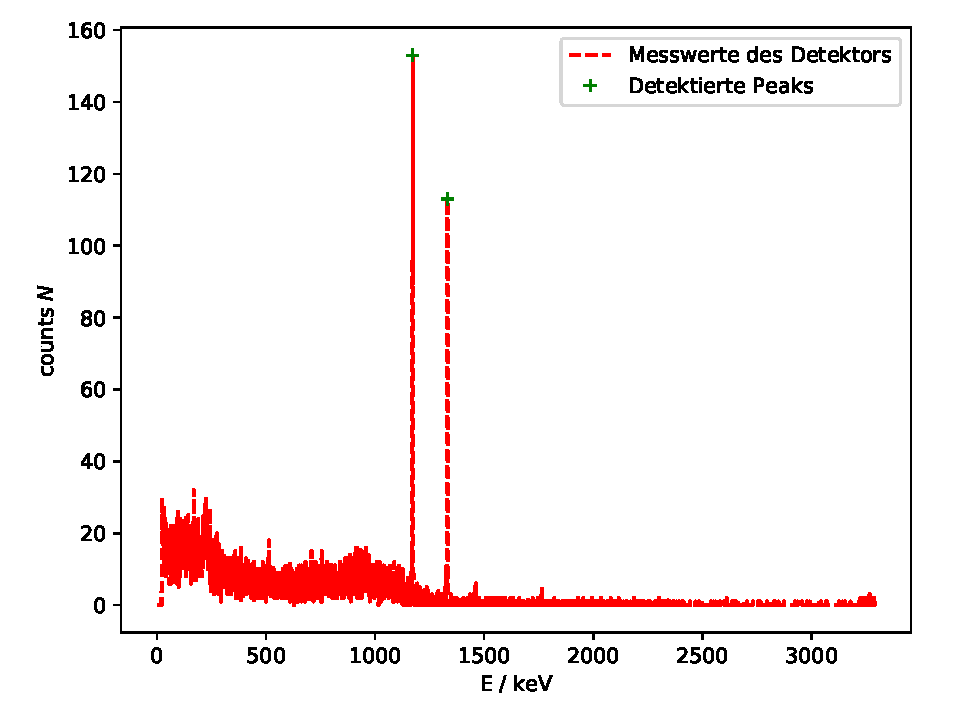
\includegraphics[scale=0.7]{unbekannterStrahler.pdf}
    \caption{Emissionsspektrum mit detektierten Peaks des unbekannten Strahlers.}
    \label{abb:unbekannt}
\end{figure}
\FloatBarrier
\begin{table}
    \centering
    \caption{Detektierte Peaks und zugeordnete Energie des unbekannten Strahlers.}
    \label{tab:unbekannt}
    \begin{tabular}{ c c c }
    \toprule
    {Bin-Index} & {counts } & {Energie $E_i$ / $\si{\kilo\electronvolt}$}\\
    \midrule
    2918 & 153.0 & 1172.66       \\
    3313 & 113.0 & 1331.38       \\
    \bottomrule
    \end{tabular}
\end{table}
\FloatBarrier

\noindent Die Energien der ermittelten Peaks werden anschließend mit Literaturwerten für verschiedene Gammastrahler verglichen. Wichtigstes Merkmal des unbekannten Gammastrahlers sind in diesem Spektrum die einzigen zwei deutlich hervorstechenden Peaks bei $\SI{1172,66}{\kilo \electronvolt}$ und $\SI{1331,38}{\kilo \electronvolt}$. Diese beiden Peaks passen sehr gut zu den beiden Peaks des $^{60}$Co, die laut Literaturangaben \cite{Q4} $\SI{1,173}{\mega \electronvolt}$ und $\SI{1,332}{\mega \electronvolt}$ betragen sollen.

\section{Diskussion}
Im ersten Teil des Versuchs konnte der lineare Zusammenhang zwischen Channel-Eingang und der Energie gut sichtbar gemacht werden.
Die große Abweichung im Fitparameter $n$ ist eventuell dadurch erklärbar, dass sich die niedrigen Peaks mit wenigen Counts nicht gut über Gaußfits approximieren lassen. Außerdem werden für die Erstellung des Fits die unkorrigierte Channelnummern verwendet.
Die sehr großen Fehler im nicht linearen Fit zur Bestimmung der Eiffizienz des Detektors lassen sich ebenso durch die schlecht zu fittenden
niedrigen Peaks erklären. Die großen Abweichungen bei der Bestimmung der Effizienz des Detektors führen dann weiterführend zu großen Abweichungen bei der Bestimmung der Aktivität von $^{133}$Ba.
Die hohe Präzision des Germanium-Detektors ist an der sehr geringen Abweichung von $\SI{0,1}{\percent}$ des detektierten Wertes für die Energie des Photopeaks vom Literaturwert \cite{Q3}. Ebenso spricht die Abweichung der Compton-Kante mit lediglich zwei Prozent vom Theoriewert für die hohe Präzision des Detektors. Die etwas höhere Abweichung des Theoriewertes für den Rückstreupeak ist dadurch zu erklären, dass der theoretische Wert nur als eine Näherung zu betrachten ist und das Ablesen des Peaks eine gewisse Ungenauigeit birgt.
Die Emissionslinien des unbekannten Strahlers konnten deutlich dargestellt und mit den Theoriewerten verglichen werden.

\printbibliography
